%!TEX root = ..\Master.tex

\subsection{Artificial Neural Network}
\subsubsection{Introduction}

Artificial neural networks are an attempt at creating a modelling how a brain works.
A network consists of neurons connected together. 
A neuron takes zero or more inputes, does some computation and gives one input as seen on figure \ref{fig:neuron}.

\begin{figure}[H]
\centering
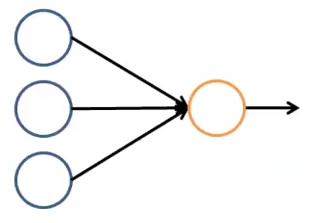
\includegraphics[scale=.5]{billeder/neuron}
\caption{A single neuron. The 3 blue circles are input units. The orange circle is the neuron.}
\label{fig:neuron}
\end{figure}

Neurons can be combined into networks as seen on figure \ref{fig:neural-network}.
How the neurons are connected is called the network architecture.
The first layer is called the input layer.
The last layer is called the output layer.
All other layers are called hidden layers.
The nodes in the network are called units.

The network on figure \ref{fig:neural-network} has 3 input units and 1 output unit which in machine learning terms means it takes 3 features and does binary classification.
To do multi-class classification, the output layer shall contain one output unit per class.

\begin{figure}[H]
\centering
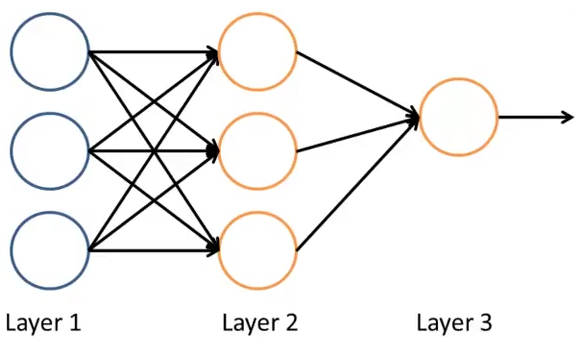
\includegraphics[scale=.5]{billeder/neural-network}
\caption{An artificial neural network with 3 layers.}
\label{fig:neural-network}
\end{figure}

Neural networks can be thought of as an extension of logistic regression.
In logistic regression we would only have layer 2 and 3, where layer 2 would contain the features.
In neural networks we can add more layers, where each new layer maps the features of the previous layer to a set of new features.
This gives more flexibility and expressive power in the model.

\subsubsection{Mathematical representation}

$a_i^{(j)}$ is the activation of unit $i$ in layer $j$, which uses the Sigmoid activation function: (TODO: show a plot. What does activation mean?)
\begin{equation}
a(x) = \dfrac{1}{1+e^{-{\Theta}^Tx}}
\end{equation}
$\Theta^{(j)}$ is a matrix of weights, controlling function mapping from layer $j$ to layer $j+1$.
If the network has $s_j$ units in layer $j$ and $s_{j+1}$ units in layer $j+1$, then $\Theta^{(j)}$ will be of dimension $s_{j+1}\times(s_j+1)$.
Each layer also contains a bias unit $a_0^{(j)}$.
The representation is illustrated on figure \ref{fig:neural-network-detailed}.

(TODO: Show how $\Theta^{(j)}$ is indexed on the figure.)

\begin{figure}[H]
\centering
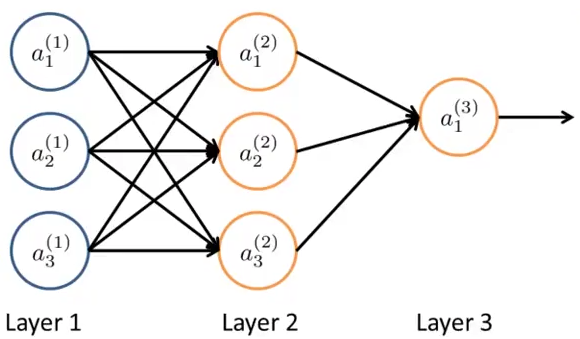
\includegraphics[scale=.5]{billeder/neural-network-detailed}
\caption{An artificial neural network with 3 layers.}
\label{fig:neural-network-detailed}
\end{figure}

The activation of a layer is defined as:

\begin{equation}
a^{(j+1)} = g(\Theta^{(j)}a^{(j)})
\end{equation}

The activation of a layer is therefore depent on the activation of the previous layer. So you have to start by activating the first layer and then propagate through the layers, hence the name of the algorithm; "forward propagation algorithm".

We can now compute the layer activations one at a time to get the output of the network on figure \ref{fig:neural-network-detailed}:
\begin{equation}
a^{(2)} = g(\Theta^{(1)}a^{(1)})
\end{equation}

\begin{equation}
a^{(3)} = g(\Theta^{(2)}a^{(2)}) = g(\Theta^{(2)} g(\Theta^{(1)}a^{(1)}))
\end{equation}

The activation of the output layer is also called:
\begin{equation}
h_\Theta(x) = a^{(3)}
\end{equation}

\subsubsection{Training the network}
Given $m$ training examples $\left\{(x^{(1)},y^{(1)}), (x^{(2)},y^{(2)}),\dots, (x^{(m)},y^{(m)}) \right\}$.
Training the neural network is an optimization problem, where the cost function $J(\Theta)$ should be minimized with respect to the weights $\Theta$.
The cost function is defined as:
\begin{equation}
\begin{split}
J(\Theta) = &-\frac{1}{m}
\left[
\sum^m_{i=1}\sum^K_{k=1}
y_k^{(i)}
log(h_\Theta(x^{(i)}))_k +
(1-y_k^{(i)})
log(1-(h_\Theta(x^{(i)}))_k)
\right] \\
&+ \frac{\lambda}{2m}
\sum^{L-1}_{k=1}
\sum^{s_l}_{i=1}
\sum^{s_{l+1}}_{j=1}
(\Theta^{(l)}_{ji})^2
\end{split}
\end{equation}

Where $L$ is the total number of layers, $s_l$ is the number of units in layer $l$, $K$ is the number of output units and $m$ is the number of training examples.

The second term of the cost function is the regularization term.

(TODO: Explain the intuition behind the cost function.)

To minimize the cost function we can use the backpropagation algorithm.

Set $\Delta^{(l)}_{ij} = 0$ (for all $l,i,j$).
$\Delta^{(l)}_{ij}$ will be used to compute
$\frac{\delta}{\delta\Theta^{(l)}_{ij}}J(\Theta)$

For $i=1to m$ (loop through trainging examples)\\
Set $a^{(1)}=x^{(i)}$ (i'th training example) \\
Perform forward propagation to compute $a^{(l)}$ for $l=2,3,\dots,L$ (activations) \\
Using $y^{(i)}$, compute $\delta^{(L)} =a^{(L)}-y^{(i)}$ (error term. $a$ is the hypothesis of the output. $y$ is the correct output/class)\\
Compute $\delta^{(L-1)},\delta^{(L-2)},\dots,\delta^{(2)}$ (backpropagation. There is no $\delta^{(1)}$ since we do not associate an error to the input layer.). \\

$\Delta^{(l)}_{ij}:=\Delta^{(l)}_{ij}+a^{(l)}_j\delta^{(l+1)}_i$ (accumulate the partial derivate terms.)  \\

END FOR \\

(TODO: Show figure of how back propagation works.)

\begin{equation}
D^{(l)}_{ij} := TODO
\end{equation}

It can be proved that:
\begin{equation}
\frac{\delta}{\delta\Theta^{(l)}_{ij}}J(\Theta) =D^{(l)}_{ij}
\end{equation}

How we use it or why we don't use it:\\

Intermediate result:\\

%------------------------------------------------